\documentclass{beamer}
\usepackage{amsmath, amssymb, amsthm}
\usepackage{graphicx, fancyhdr}
\usepackage{mdframed} % Add this to the preamble
\usepackage{xcolor} % Ensure xcolor is included
\definecolor{Teal}{HTML}{23373B} % Define the color
\definecolor{darkGreen}{rgb}{0.0, 0.5, 0.0}  % Define dark green color
% Theme choice
\usetheme{metropolis} % Modern and clean layout
% Custom Block Colors
\usepackage{xcolor}
\setbeamercolor{block title}{fg=white, bg=Teal!90} % Block title color
\setbeamercolor{block body}{fg=black, bg=gray!15}  % Block body color

\newtheorem{conjecture}{Conjecture}
% Footer settings
\setbeamertemplate{footline}{
  \leavevmode\hbox{\begin{beamercolorbox}[wd=\paperwidth,ht=3ex,dp=2ex]{author in head/foot}%
      \hspace{1em} {M. J. Moghaddas Mehr}
      \, \textbar \,
      \insertshorttitle \,
      \textbullet \, 
      \insertsection \, 
      \hfill \insertframenumber{}/\inserttotalframenumber{} \hspace{.5em}
  \end{beamercolorbox}
  }
}

% Title Page Details
\title{Isomorphism in Union-Closed Sets}
\author{Mohammad Javad Moghaddas Mehr}
\date{Cincinnati – March 2025}

\begin{document}

% Title Slide
\begin{frame}
	\titlepage
\end{frame}

% Slide 2: History of the Union-Closed Conjecture
\begin{frame}{History}
	In 1979, Péter Frankl proposed a famous conjecture about finite union-closed families.
	He stated that in every such family, there exists an element that appears in at least half of the sets.
	Despite significant efforts, the problem has remained unsolved for more than four decades.
	\vfill
	\vfill
	\begin{block}{Union-Closed Conjecture (Frankl, 1979)}
		Let \(\mathcal{K} \subseteq 2^{[n]}\) be a union-closed family of sets.
		Then there exists an element \(i \in \bigcup \mathcal{K}\) such that: \(|\mathcal{K}| \leq 2|\mathcal{K}^i|\),
		where
		\[
			\mathcal{K}^i = \{A \in \mathcal{K} \mid i \in A\}.
		\]
	\end{block}

\end{frame}


\begin{frame}{Examples}
	\textbf{Example 1:} Consider the family of sets:
	\[
		\mathcal{K} = \{\varnothing, \{1\}, \{1,2\}, \{2,3,4\}, \{1,2,3,4\}\}
	\]
	The desired elements are \(1\) or \(2\).


	\vfill

	\textbf{Example 2:} Consider the family of sets:
	\[
		\mathcal{K} = \{\varnothing, \{a\}, \{b\}, \{a,b\}\}
	\]
	The desired elements are \(a\) or \(b\).
\end{frame}




\begin{frame}
	\begin{itemize}
		\item 	If a union-closed family satisfies Frankl’s conjecture, does every isomorphic family also satisfy it?
		\item Does isomorphic families have members with same frequency count?
		\item Are all member of the families have a counterpart with same frequency count?

	\end{itemize}

	\vfill
	\begin{Definition}
		Let \( \mathcal{K}_1 \) and \( \mathcal{K}_2 \) be union-closed families of sets.
		A bijective mapping \( h: \mathcal{K}_1 \to \mathcal{K}_2 \) is called a \textbf{Isomorphism} if, for all
		\( A_1, A_2 \in \mathcal{K}_1 \), the following property holds:
		\[
			h(A_1 \cup A_2) = h(A_1) \cup h(A_2).
		\]
	\end{Definition}
\end{frame}

\begin{frame}
	\begin{itemize}
		\item[\textcolor{red}{\textbf{X}}] Are all members of the families paired with a counterpart of the same frequency count?
	\end{itemize}

	\pause
	\vfill
	\begin{center}
		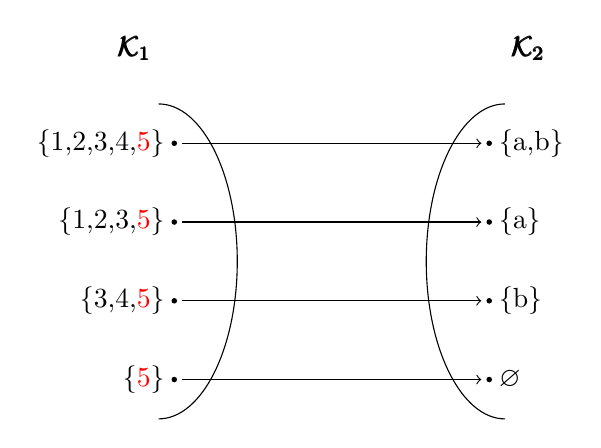
\begin{tikzpicture}[scale=1]
			\draw[thin] (3.2,2) arc[start angle=90, end angle=270, x radius=1, y radius=2]; % X on the right
			\draw[thin] (-1.2,-2) arc[start angle=-90, end angle=90, x radius=1, y radius=2]; % Y on the left
			% Labels for sets
			\node at (-1.5,2.7) {\(\pmb{\mathcal{K}_1}\)};
			\node at (3.5,2.7) {\(\pmb{\mathcal{K}_2}\)};

			% Elements in X (now enclosed in sets)
			\node[left] at (-1,1.5) {\{1,2,3,4,\textcolor{red}{5}\}};
			\node[left] at (-1,0.5) {\{1,2,3,\textcolor{red}{5}\}};
			\node[left] at (-1,-0.5) {\{3,4,\textcolor{red}{5}\}};
			\node[left] at (-1,-1.5) {\{\textcolor{red}{5}\}};

			% Elements in Y (now enclosed in sets)
			\node[right] at (3,1.5) {\{a,b\}};
			\node[right] at (3,0.5) {\{a\}};
			\node[right] at (3,-0.5) {\{b\}};
			\node[right] at (3,-1.5) {\(\varnothing\)};


			% Draw mappings
			\draw[->, thin] (-.9,1.5) -- (2.9,1.5);
			\draw[->, thin] (-.9,0.5) -- (2.9,0.5);
			\draw[->, thin] (-.9,-0.5) -- (2.9,-0.5);
			\draw[->, thin] (-.9,-1.5) -- (2.9,-1.5);

			% Draw points in X
			\foreach \y in {1.5,0.5,-0.5,-1.5}
			\fill (-1,\y) circle (1pt);

			% Draw points in Y
			\foreach \y in {1.5,0.5,-0.5,-1.5}
			\fill (3,\y) circle (1pt);
		\end{tikzpicture}
	\end{center}

\end{frame}

\begin{frame}

	\begin{itemize}
		\item[\textcolor{orange}{\textbf{?}}]	If a union-closed family satisfies Frankl’s conjecture, does every isomorphic family also satisfy it?
			\pause

		\item[\textcolor{darkGreen}{\textbf{\checkmark}}]  Does isomorphic families have members with same frequency count?
	\end{itemize}
	\vfill


	\pause
	\begin{center}
		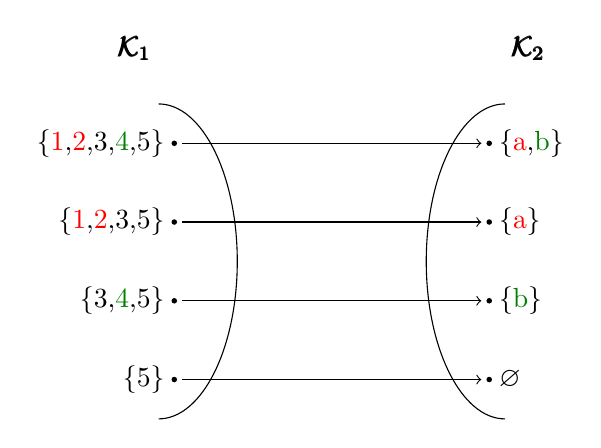
\begin{tikzpicture}[scale=1]
			\draw[thin] (3.2,2) arc[start angle=90, end angle=270, x radius=1, y radius=2]; % X on the right
			\draw[thin] (-1.2,-2) arc[start angle=-90, end angle=90, x radius=1, y radius=2]; % Y on the left
			% Labels for sets
			\node at (-1.5,2.7) {\(\pmb{\mathcal{K}_1}\)};
			\node at (3.5,2.7) {\(\pmb{\mathcal{K}_2}\)};

			% Elements in X (now enclosed in sets)
			\node[left] at (-1,1.5) {\{\textcolor{red}{1},\textcolor{red}{2},3,\textcolor{darkGreen}{4},5\}};
			\node[left] at (-1,0.5) {\{\textcolor{red}{1},\textcolor{red}{2},3,5\}};
			\node[left] at (-1,-0.5) {\{3,\textcolor{darkGreen}{4},5\}};
			\node[left] at (-1,-1.5) {\{5\}};

			% Elements in Y (now enclosed in sets)
			\node[right] at (3,1.5) {\{\textcolor{red}{a},\textcolor{darkGreen}{b}\}};
			\node[right] at (3,0.5) {\{\textcolor{red}{a}\}};
			\node[right] at (3,-0.5) {\{\textcolor{darkGreen}{b}\}};
			\node[right] at (3,-1.5) {\(\varnothing\)};


			% Draw mappings
			\draw[->, thin] (-.9,1.5) -- (2.9,1.5);
			\draw[->, thin] (-.9,0.5) -- (2.9,0.5);
			\draw[->, thin] (-.9,-0.5) -- (2.9,-0.5);
			\draw[->, thin] (-.9,-1.5) -- (2.9,-1.5);

			% Draw points in X
			\foreach \y in {1.5,0.5,-0.5,-1.5}
			\fill (-1,\y) circle (1pt);

			% Draw points in Y
			\foreach \y in {1.5,0.5,-0.5,-1.5}
			\fill (3,\y) circle (1pt);
		\end{tikzpicture}
	\end{center}
\end{frame}

\begin{frame}{Thank You!}
	\textbf{Any Questions?}
	\begin{itemize}
		\item Email: m.moghadas11235@gmail.com
		\item Paper available on ArXiv.
	\end{itemize}
\end{frame}

\end{document}
